\chapter{Results}
% This will be the main part. It should address the research questions, in a suitable structure: for example, one section per research question, or following the data science pipeline (data engineering --> modeling --> benchmarking --> deployment etc.). The concrete structure will depend on your topic.
% Avoid code details here, just explain the general structure of your approach: what has been done and why? Report the results of data analyses and model statistics and give interpretations. Code parts will be provided in the Appendix as commented notebooks.
% As mentioned, a mandatory part of your results is a suitable deployment, at least as a concept.


\section{Exploratory Data Analysis}
This section presents the \ac{EDA}, with a particular focus on aspects relevant to the research questions.
\autoref{fig:target-water-level-history} provides an overview of the daily maximum water level over the full available period, together with weekly precipitation totals and the train/test split.
\autoref{fig:target-water-level-distribution} illustrates the distribution of water level measurements at the target station to examine the frequency and magnitude of high water events.
Data availability is examined in \autoref{fig:station-monthly-data-completeness}, which shows the availability of water level measurements across all eligible stations and the proportion of rows at the target station for which all required features are available.
To investigate the potential contribution of neighboring stations, \autoref{fig:upstream-cross-correlation-heatmap} presents the Pearson correlation between upstream stations and the target station for lags of 0--72 hours.
Finally, \autoref{fig:weather-future-change-spearman} presents the Spearman correlation between precipitation sums, temperature means and subsequent water level changes at the target station, providing an indication of the relationship between weather conditions and future water level development.

As seen in \autoref{fig:target-water-level-history} there is quite some variability in the water level over time. The majority of the daily maximum stays below the alarm threshold of 545 cm. Values above the threshold are rare and short lived, which is to be expected. The highest water level observed is on the 15\textsuperscript{th} of September 2024, with a value of 761 cm. This value is in the test set which means that the model will be evaluated on a previously unseen extreme event, the model will likely not be able to predict this extreme value accurately. The highest weekly water level sum is about 274 mm, which has a z-score of 14.56. The mean weekly precipitation sum is about 13 mm. As expected there is no real trend, neither upward nor downward, in the water level over time. However high precipitation and high water levels do not always coincide, as seein in on the second highest water level measured at the 4\textsuperscript{th} of June 2024 (the spike before the highest spike). There the precipitation sum is relatively low (about 37 mm). This is also somewhat expected, as the water level is not only influenced by the precipitation at the target station, but also by all upstream precipitation.
\begin{figure}[htbp]
  \centering
  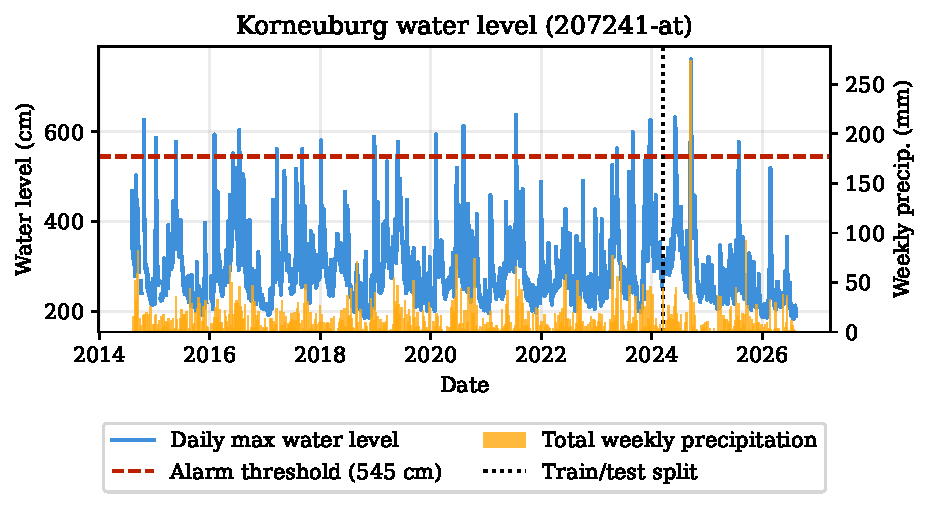
\includegraphics[width=\textwidth]{figures/target_water_level_history.pdf}
  \caption{Daily maximum water level at station 207241-at (in Korneuburg) over the full available period with weekly precipitation totals and the train/test split.}\label{fig:target-water-level-history}
\end{figure}

\autoref{fig:target-water-level-distribution} shows the distribution of observed hourly water levels at the target station. The distribution is right-skewed, with a long tail towards higher water levels. The first quartile is at 229 cm, the median is at 262 cm, and the third quartile is at 310 cm. The alarm threshold of 545 cm is far above the third quartile, values above the threshold are rare, with only 760 observations (0.75\% of the total) exceeding the threshold. 
% \autoref{fig:target-water-level-distribution}: Number of observations above alarm threshold: 760 (0.75%) Quartiles: Q1=229.00, Q2=262.00, Q3=310.00
\begin{figure}[htbp]
  \centering
  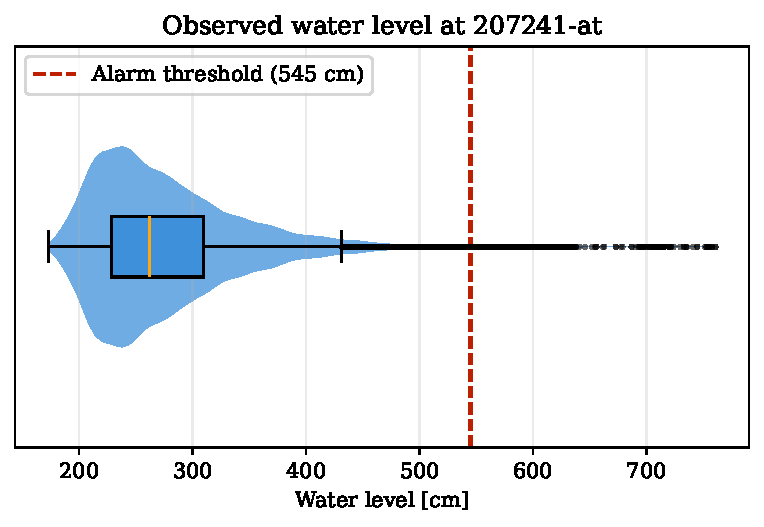
\includegraphics[width=\textwidth]{figures/target_water_level_distribution.pdf}
  \caption{Distribution of observed hourly water levels at the target station.}\label{fig:target-water-level-distribution}
\end{figure}


\autoref{fig:station-monthly-data-completeness} outlines the monthly availability of water level measurements across all eligible stations, as well as the proportion of rows that are eligible for use in the model. 207340-at, 207027-at and 207019-at have a later start date than the other stations, they are missing all measurements before mid 2015. Overall the availability of water level measurements is quite good, with the lowest availability being about 89\%. There are also some patterns in the missingness of the data. For example late 2015 and early 2016 there are some months with lower availability, of the same three stations. The reason could be that there is was an issue at the measurement station operator's side, or that FloodAlert was not able to fetch the data for some other reason (e.g. outage of their system). The proportion of rows that are eligible for use in the model training is comparatively low, since it requires that all features are available. This is due to several factors, the first one being that the the target must not be null for the entire 24 hour forecast horizon. A single null value in the target will make the many rows ineligible. Furthermore, all features must not be null for for the row to be eligible. Nevertheless the total number of eligible rows is still quite high with about 70,000 rows.
\begin{figure}[htbp]
  \centering
  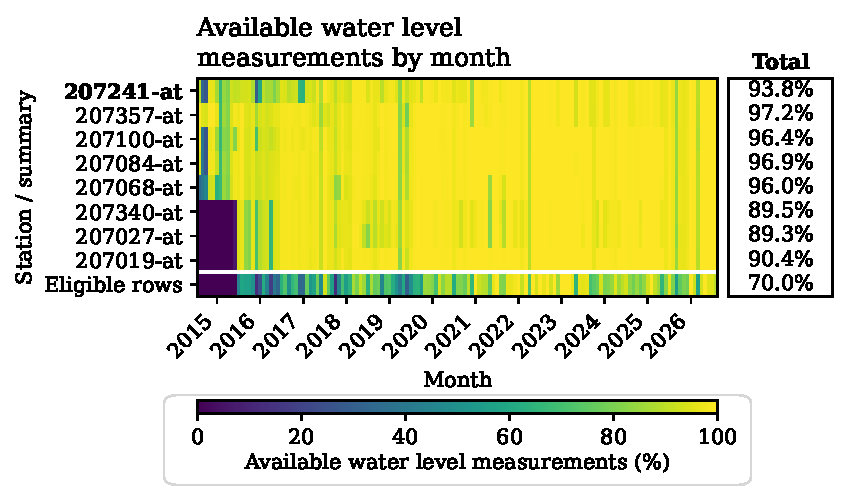
\includegraphics[width=\textwidth]{figures/station_monthly_data_completeness.pdf}
  \caption{Monthly available water level measurements and eligible rows for upstream stations (interpolated measurements count as missing).}\label{fig:station-monthly-data-completeness}
\end{figure}


The Pearson cross-correlation between upstream stations and the target station for lags of 0--72 hours is shown in \autoref{fig:upstream-cross-correlation-heatmap}. The plot indicates how many hours later the target station's measurements are most strongly correlated with the upstream stations' measurements. A lag of e.g. 2 hours before Korneuburg means that the upstream station's measurement at time $t$ is compared with Korneuburg's measurement two hours later ($t+2$). The circles in the plot mark the highest correlation for each station, which provides an indication of the propagation delay of water level changes. The stations are sorted by the distance to the target station, with the closest station at the top. With increasing lags the correlation decreases with the lowest correlation at 72 hours being between 0.66 and 0.75 All stations have their highest correlation with Kroneuburg at a lag of 2--7 hours. Except 207084-at, all stations also have a very high correlation of 0.95 or higher. It is not clear why the highest correlation for 207084-at is only 0.89. The lag associated with the maximum correlation generally increases for stations farther upstream. Station 207084-at is an exception to this pattern, reaching its maximum correlation at a lag of 7 hours, while the following two stations, both peak at a lag of 6 hours.
\begin{figure}[htbp]
  \centering
  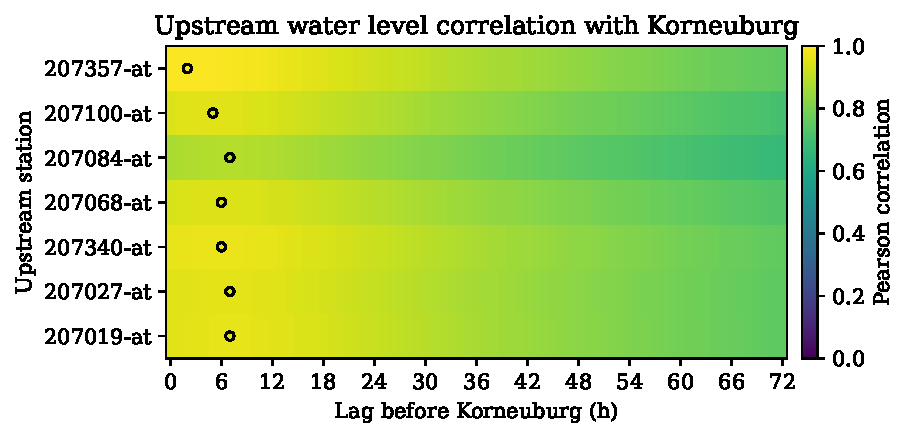
\includegraphics[width=\textwidth]{figures/upstream_cross_correlation_heatmap.pdf}
  \caption{Pearson cross-correlation between upstream stations and Korneuburg for lags of 0-72 hours. Positive lag means the upstream measurement leads Korneuburg; circles mark each station's peak.}\label{fig:upstream-cross-correlation-heatmap}
\end{figure}

The heatmap in \autoref{fig:weather-future-change-spearman} shows the Spearman correlation between precipitation sums, temperature means and subsequent water level changes at the target station. There is virtually no linear correlation between the temperature and future water level changes, with the highest correlation being 0.04 showing no monotonic relationship between the mean temperature and the future water level changes. The precipitation sums show a larger weak correlation with future water level changes, with the highest correlation being 0.26. Increased precipitation over the previous 6 and 24 hours is associated with the strongest subsequent water level changes  12 or 24 hours later. The correlation pattern suggests a delayed association between recent precipitation and water level changes. The weak negative correlation for the 72-hour precipitation sum at the 48-hour horizon may indicate that the water level has already risen due to earlier rainfall and is beginning to fall again. Additionally, the long 72-hour window makes it difficult to determine when exactly the precipitation occurred.
\begin{figure}[htbp]
  \centering
  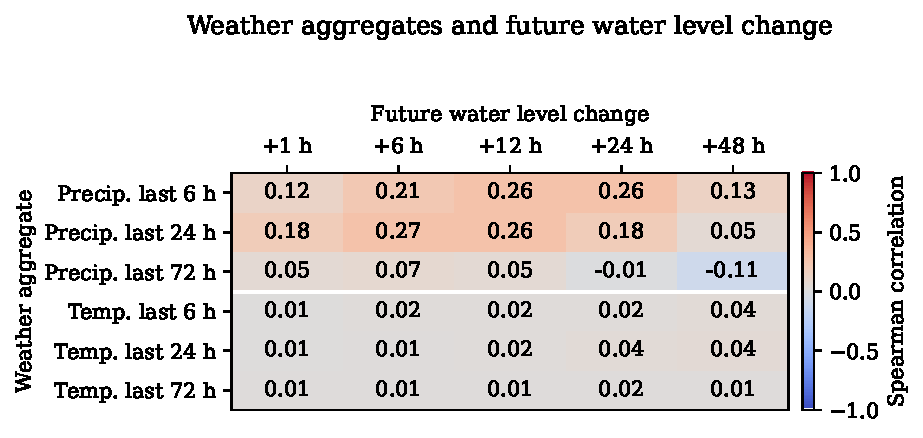
\includegraphics[width=\textwidth]{figures/weather_future_change_spearman.pdf}
  \caption{Spearman correlations between precipitation sums / temperature means and future water level changes at the target station.}\label{fig:weather-future-change-spearman}
\end{figure}



% TODO TAlk about hyperparameter spaces searched
\section{Model Performance}
Compare all model performances and select best model
\section{Feature Effects}
Investigate feature importance and effects on the model performance

\section{Forecast Analysis}
In depth analysis of the forecast performance (e.g.) e.g. performance over lead time, ... for the best/chosen model

\section{Deployment}
Deployment (Docker + FastAPI)
